\documentclass[../basic_graph_theory.tex]{subfiles}

\begin{document}

\chapter{Basic Definitions}
\setcounter{chapter}{1} % Set chapter counter
\setcounter{section}{0}
\setcounter{equation}{0}
\setcounter{figure}{0}

\section{Notation and Preliminaries}
\begin{Def}{Graph}{}
  A (simple) graph $G = (V, E)$ consists of a finite vertex set $V$ and an edge set $E \subseteq \binom{V}{2}$.
\end{Def}

Before delving deeper, let's establish definitions for various classes of graphs.

\begin{enumerate}
  \item \textbf{Undirected Graph}: An undirected graph is characterized by edges $(x, y)$ being equivalent to $(y, x)$.

        \begin{figure}[hbt!]
          \centering
          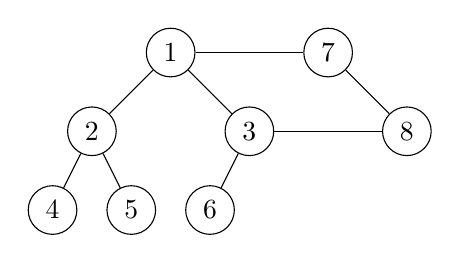
\begin{tikzpicture}[every node/.style={circle, draw, minimum size=5mm}]
            % Tree part
            \node (1) at (0,0) {1};
            \node (2) at (-1,-1) {2};
            \node (3) at (1,-1) {3};
            \node (4) at (-1.5,-2) {4};
            \node (5) at (-0.5,-2) {5};
            \node (6) at (0.5,-2) {6};

            \draw (1) -- (2);
            \draw (1) -- (3);
            \draw (2) -- (4);
            \draw (2) -- (5);
            \draw (3) -- (6);

            % Cycle part
            \node (7) at (2,0) {7};
            \node (8) at (3,-1) {8};

            \draw (7) -- (8);
            \draw (8) -- (3);
            \draw (1) -- (7);
          \end{tikzpicture}
          \caption{Undirected graph}
          \label{fig:undirected}
        \end{figure}
  \item \textbf{Directed Graph}: A directed graph or digraph $ G = (V, E) $ represents edges as ordered pairs of vertices, i.e., $ E \subseteq V \times V $.
        \begin{figure}[hbt!]
          \centering
          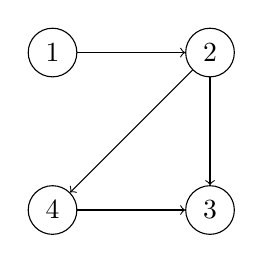
\begin{tikzpicture}[->, every node/.style={circle, draw, minimum size=5mm}]

            % Nodes
            \node (1) at (0,0) {1};
            \node (2) at (2,0) {2};
            \node (3) at (2,-2) {3};
            \node (4) at (0,-2) {4};

            % Directed edges
            \draw (1) -> (2);
            \draw (2) -> (3);
            \draw (2) -> (4);
            \draw (4) -> (3);

          \end{tikzpicture}
          \caption{Directed graph}
          \label{fig:directed}
        \end{figure}
  \item \textbf{Multigraph}: A multigraph $ G = (V, E) $ where there can be more than one edge between any given vertices, i.e., $ E \subseteq \binom{V}{2} $ is a multiset.
        \begin{figure}[hbt!]
          \centering
          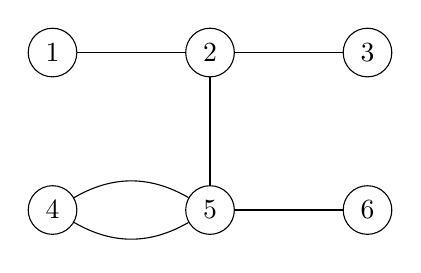
\begin{tikzpicture}[>=stealth, every node/.style={circle, draw, minimum size=5mm}]

            % Nodes
            \node (1) at (0,0) {1};
            \node (2) at (2,0) {2};
            \node (3) at (4,0) {3};
            \node (4) at (0,-2) {4};
            \node (5) at (2,-2) {5};
            \node (6) at (4,-2) {6};

            % Multiedges
            \draw (1) -- (2);
            \draw (2) -- (3);
            \draw (2) -- (5);
            \draw (5) -- (6);
            \draw (4) to[bend right=30] (5); % Curved multiedge
            \draw (5) to[bend right=30] (4); % Curved multiedge

          \end{tikzpicture}
          \caption{Multigraph}
          \label{fig:multigraph}
        \end{figure}
  \item \textbf{Pseudograph}: A pseudograph \( G = (V, E) \) allows loops and multiple edges. Formally, \( E \) is a subset of pairs of distinct vertices in \( V \) (\( \binom{V}{2} \)) and pairs with identical elements (\( \left\{ (v, v) \mid v \in V \right\} \)), i.e., \( E \subseteq \binom{V}{2} \cup \left\{ (v, v) \mid v \in V \right\} \).
        \begin{figure}[hbt!]
          \centering
          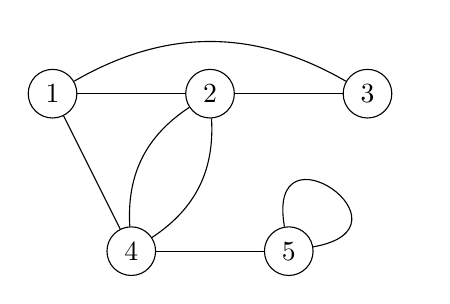
\begin{tikzpicture}[>=stealth, every node/.style={circle, draw, minimum size=5mm}]

            % Nodes
            \node (1) at (0,0) {1};
            \node (2) at (2,0) {2};
            \node (3) at (4,0) {3};
            \node (4) at (1,-2) {4};
            \node (5) at (3,-2) {5};

            % Pseudograph with self-loops
            \draw (1) -- (2);
            \draw (1) -- (4);
            \draw (2) -- (3);
            \draw (2) to[bend right] (4);
            \draw (2) to[bend left] (4);
            \draw (3) to[bend right=30] (1);
            \draw (4) -- (5);
            \draw (5) to [out=10, in=100, looseness=8] (5);
          \end{tikzpicture}
          \caption{Pseudograph}
          \label{fig:pseudograph}
        \end{figure}
  \item \textbf{Hypergraph}: A hypergraph \( G = (V, E) \) has edges that can be any subset of vertices, expressed as \( E \subseteq 2^V \).
        \begin{figure}[hbt!]
          \centering
          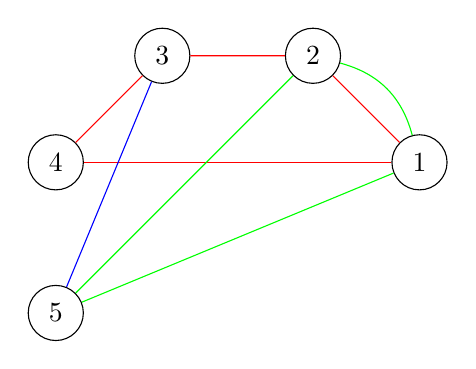
\begin{tikzpicture}[every node/.style={circle, draw, fill=white, minimum size=7mm}]

            % Nodes
            \foreach \i in {1,...,5}
            \node (\i) at ({45*\i - 22.5}:2.5) {\i};

            % Hyperedges with colors and bending
            \draw[red] (1) -- (2) -- (3) -- (4) -- cycle;
            \draw[red] (1) -- (4) -- cycle;
            \draw[green] (1) -- (5) -- (2) edge[bend left] (1);
            \draw[blue] (3) -- (5) -- cycle;
          \end{tikzpicture}
          \caption{Hypergraph $ \left( [5], \left\{ \{ 1, 2, 3, 4 \}, \{ 1, 2, 5 \}, \{ 3, 5 \} \right\} \right) $}
          \label{fig:hypergraph}
        \end{figure}
  \item \textbf{Infinite Graph}: A graph where the set $V$ or $E$ is infinite.
\end{enumerate}

\section{Important Terminologies}
\begin{Def}{Neighbourhood}{}
  The neighbourhood of a vertex $v$ in graph $G$, denoted by $N(v)$, represents the set of vertices adjacent to $v$: $N(v) = \left\{x \in V(G) \mid \{v,x\} \in E(G)\right\}$.
\end{Def}

Let's introduce some basic concepts.

\begin{Def}{Order and Size}{}
  The order of the graph, denoted by $|V(G)|$, is the cardinality of $V(G)$. Similarly, the size of the graph, denoted by $|E(G)|$, is the cardinality of $E(G)$.
\end{Def}

We introduce two more notations:

\begin{itemize}
  \item The maximum degree of a graph $G$ is denoted by $\Delta(G)$: $\Delta(G) = \max\{\deg(v) \mid v \in V(G)\}$.
  \item The minimum degree of a graph $G$ is denoted by $\delta(G)$: $\delta(G) = \min\{\deg(v) \mid v \in V(G)\}$.
\end{itemize}

Now, let's state one of the famous and basic theorems.

\begin{Thm}{}{}
  \label{ref:3}
  In a graph $G$, the sum of the degrees of vertices is equal to twice the number of edges:
  \[ 2 |E(G)| = \sum_{v \in V(G)}\deg(v) \]
\end{Thm}

\begin{proof}
  Easy exercise. Try to double count the set $ \left\{ (v, e) \in V \times E \mid v \in e \right\} $.
\end{proof}

We will now introduce two very useful concepts: \textit{vertex deletion} and \textit{edge deletion}.

The notation $G - v$ denotes the graph obtained by excluding vertex $v$ and all its incident edges from $G$, expressing the concept of vertex deletion. This can be formally described as \[ G - v = (V(G) \setminus \{v\}, E(G) \setminus \{e : v \in e\}) \]

\

Similarly, $G - e$ signifies the graph resulting from the removal of a specific edge $e$ in $G$, while keeping its original end vertices intact. In other words, \[ G - e = (V(G), E(G) \setminus \{e\}) \]

\

Additionally, the notation $G / e$ denotes the graph obtained by merging the end vertices $v_1$ and $v_2$ of edge $e = \{v_1, v_2\}$ into a single vertex $v$. In the graph $G$, every edge incident on either $v_1$ or $v_2$ is now incident on $v$ in the updated notation $G/e$, which can be formally expressed as
\[ G / e = (V(G), E(G)) / \sim_{e} \]
where $\sim_{e}$ denotes the equivalence relation $v_1 \sim_{e} v_2$ .

\

We now define the concepts of connectedness and cut sets.

\begin{Def}{Connected Graph}{}
  A graph \( G \) is connected if, for every pair of vertices \( u, v \) in \( G \), there exists a sequence of edges \( e_1, \dots, e_k \) such that \( u \in e_1 \), \( v \in e_k \), and the intersection size \( \abs{e_i \cap e_{i+1}} = 1 \) for all \( i \).
\end{Def}

\begin{Def}{Connected Component}{}
  Let \( G = (V, E) \) be a graph. A connected component of \( G \) is a maximal subgraph \( G' = (V', E') \) of \( G \), such that:
  \begin{itemize}
    \item Every vertex in \( V' \) is connected to every other vertex in \( V' \) by a path in \( G' \).
    \item There is no vertex in \( V - V' \) that can be added to \( V' \) without violating the previous condition.
  \end{itemize}
\end{Def}

\begin{Def}{Cut Vertex}{}
  Let \( G = (V, E) \) be a graph. A vertex \( v \) in \( V \) is a cut vertex if and only if the removal of \( v \) from \( G \) results in an increase in the number of connected components of \( G \).
\end{Def}

\begin{Def}{Cut Edge or Bridge}{}
  Let \( G = (V, E) \) be a graph. An edge \( e \in E \) is a cut edge or bridge if and only if the removal of \( e \) from \( G \) results in an increase in the number of connected components of \( G \).
\end{Def}

\begin{Def}{Vertex Cut Set}{}
  Let \( G = (V, E) \) be a graph. A proper subset \( S \subset V(G) \) is a vertex cut set if and only if the removal of \( S \) from \( G \) results in a disconnected graph.
\end{Def}

\begin{Def}{Connectivity}{}
  Let \( G = (V, E) \) be a graph. The connectivity of \( G \), denoted by \( \kappa(G) \), is defined as the minimum size of a cut set of \( G \).
\end{Def}

Next, we go on to define a few more types of graphs.

\begin{enumerate}
  \item \textbf{Complement of a Graph}: The complement of a graph $G$ is the graph on $n$ vertices, where all possible vertices $(x,y) \notin E(G)$.
  \item \textbf{Line Graph of a Graph}: The line graph $L(G)$, where each edge in $G$ is represented by a vertex in $L(G)$, and an edge exists between two vertices of $L(G)$ if the corresponding edges in $G$ share a vertex.
  \item \textbf{Regular Graph}: A graph whose every vertex has equal degree.
  \item \textbf{Bipartite Graph}: A graph whose vertices can be divided into two partite sets $X$ and $Y$, such that no two vertices in a partite set are adjacent to each other.
  \item \textbf{Subgraph}: A graph $H$ is called the subgraph of a graph $G$ if $V(H) \subseteq V(G)$ and $E(H) \subseteq E(G)$.
\end{enumerate}

\begin{Def}{Graph Homomorphism and Isomorphism}{}
  Suppose $G$ and $H$ are two graphs. A function $\phi : V(G) \to V(H)$ is a \textit{graph homomorphism} if $\left\{ x, y \right\} \in E(G)$ implies $\{\phi(x), \phi(y)\} \in E(H)$. $\phi$ is an \textit{isomorphism} if $\phi$ is a bijection, and $\left\{ x, y \right\} \in E(G)$ if and only if $\{\phi(x), \phi(y)\} \in E(H)$, i.e., $\phi$ and $\phi^{-1}$ are graph homomorphisms. $G$ and $H$ are \textit{isomorphic} ($G \cong H$) if there exists an isomorphism between $G$ and $H$. An \textit{automorphism} is an isomorphism $\phi : G \to G$ from a graph $ G $ to itself.
\end{Def}

That concludes the basic definitions we will be needing. Further on, we will introduce various interesting ideas, and in our Random Graphs WRP, these ideas will be of essence.

\end{document}
